% 例 2：坐标系中以原点为位似中心 k=1/2，正向、反向各一组
\documentclass[tikz,border=4pt]{standalone}
\usepackage{ctex}
\usepackage{amsmath}
\usetikzlibrary{arrows.meta}
\begin{document}
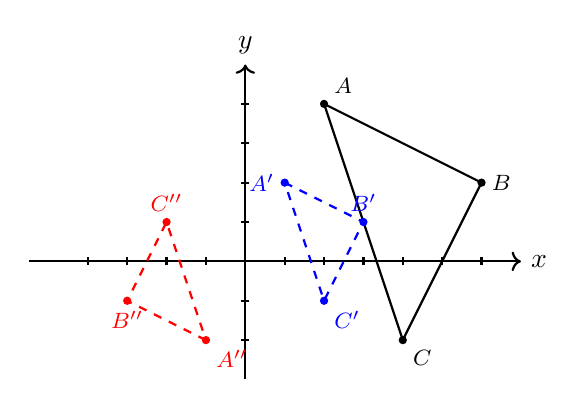
\begin{tikzpicture}[scale=0.5, thick]
  \draw[->] (-5.5,0) -- (7,0) node[right]{$x$};
  \draw[->] (0,-3) -- (0,5) node[above]{$y$};
  \foreach \i in {-4,-3,-2,-1,1,2,3,4,5,6} \draw (\i,0.1) -- (\i,-0.1);
  \foreach \i in {-2,-1,1,2,3,4} \draw (0.1,\i) -- (-0.1,\i);

  % 原图形 A(2,4) B(6,2) C(4,-2)
  \coordinate (A) at (2,4);
  \coordinate (B) at (6,2);
  \coordinate (C) at (4,-2);
  \draw (A) -- (B) -- (C) -- cycle;
  \fill (A) circle (3pt); \fill (B) circle (3pt); \fill (C) circle (3pt);
  \node[above right] at (A) {\footnotesize $A$};
  \node[right] at (B) {\footnotesize $B$};
  \node[below right] at (C) {\footnotesize $C$};

  % 正向 k=1/2: A'(1,2) B'(3,1) C'(2,-1)
  \coordinate (Ap) at (1,2);
  \coordinate (Bp) at (3,1);
  \coordinate (Cp) at (2,-1);
  \draw[blue, dashed] (Ap) -- (Bp) -- (Cp) -- cycle;
  \fill[blue] (Ap) circle (3pt); \fill[blue] (Bp) circle (3pt); \fill[blue] (Cp) circle (3pt);
  \node[left, blue] at (Ap) {\footnotesize $A'$};
  \node[above, blue] at (Bp) {\footnotesize $B'$};
  \node[below right, blue] at (Cp) {\footnotesize $C'$};

  % 反向 k=-1/2: A''(-1,-2) B''(-3,-1) C''(-2,1)
  \coordinate (App) at (-1,-2);
  \coordinate (Bpp) at (-3,-1);
  \coordinate (Cpp) at (-2,1);
  \draw[red, dashed] (App) -- (Bpp) -- (Cpp) -- cycle;
  \fill[red] (App) circle (3pt); \fill[red] (Bpp) circle (3pt); \fill[red] (Cpp) circle (3pt);
  \node[below right, red] at (App) {\footnotesize $A''$};
  \node[below, red] at (Bpp) {\footnotesize $B''$};
  \node[above, red] at (Cpp) {\footnotesize $C''$};
\end{tikzpicture}
\end{document}
